\graphicspath{{./Installation/eps/}} 

\cleardoublepage
%%%%%%%%%%%%%%%%%%%%%%%%%%%%%%%%%%%%%%%%%%%%%%%%%%%%%%%%%%%%%%%%%%%%%%%%%%%%%%%%%%%%%%%%%%%%%%%%%%%%%%%%%%%%%%%%%%%%%%%%%%%%

\chapter{Installationshinweise}

\wspwin\ wird f�r die Betriebssysteme Windows NT, 2000 und XP vertrieben.

%%%%%%%%%%%%%%%%%%%%%%%%%%%%%%%%%%%%%%%%%%%%%%%%%%%%%%%%%%%%%%%%%%%%%%%%%%%%%%%%%%%%%%%%%%%%%%%%%%%%%%%%%%%%%%%%%%%%%%%%%%%%

%%%%%%%%%%%%%%%%%%%%%%%%%%%%%%%%%%%%%%%%%%%%%%%%%%%%%%%%%%%%%%%%%%%%%%%%%%%%%%%%%%%%%%%%%%%%%%%%%%%%%%%%%%%%%%%%%%%%%%%%%%%%
\section{Installation}
%%%%%%%%%%%%%%%%%%%%%%%%%%%%%%%%%%%%%%%%%%%%%%%%%%%%%%%%%%%%%%%%%%%%%%%%%%%%%%%%%%%%%%%%%%%%%%%%%%%%%%%%%%%%%%%%%%%%%%%%%%%%

Ab der Version \wspwin{~4.0} werden die Windows-Oberfl\"{a}chen, das Berechnungsprogramm sowie evtl. Zusatzprogramme in einem
Installationsvorgang von CD-ROM auf Ihrem Rechner installiert. Davon ausgenommen sind allerdings \wspwin{}-Plotter und
\wspwin{}-Mapper, die separat installiert werden m\"{u}ssen. Starten Sie \"{u}ber den Windows-Explorer die Datei
\datei{setup.exe}. Der Installationsmanager geleitet Sie nun durch die Programminstallation.
\begin{figure}
   \centering
   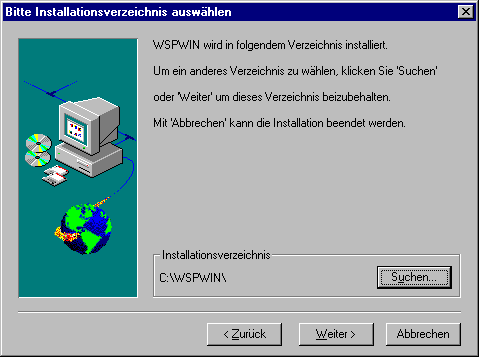
\includegraphics[width=0.9\linewidth]{Installationspfad}
   \caption{Auswahl des Installationspfades}
   \label{Installation Abb Installationspfad}
\end{figure}
Die Installation bietet standardm\"{a}{\ss}ig das Verzeichnis \datei{C:\textbackslash WSPWIN} als Installationsverzeichnis an.
Soll die Installation in einem anderen Verzeichnis erfolgen, dr\"{u}cken sie \schalter{Suchen...} und w\"{a}hlen das neue
Installationsverzeichnis oder geben den Pfad von Hand ein.

Grunds\"{a}tzlich bestehen \"{u}ber das Installationsprogramm die im folgenden beschriebenen vier M\"{o}glichkeiten der Installation:
\begin{figure}
   \centering
   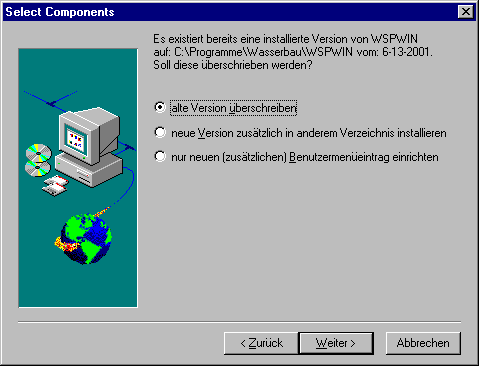
\includegraphics[width=0.9\linewidth]{Optionen}
   \caption{Installationsoptionen}
   \label{Installation Abb Optionen}
\end{figure}

\subsubsection{Erstinstallation} Es wurde keine \wspwin{}-Programmdatei vom Setup-Programm vorgefunden. Sie haben die
M\"{o}glichkeit zu entscheiden, ob nur \wspwin{} oder auch HYDRA-Programme (bei Erwerb) bzw. Demoprojekte installiert werden
sollen.

\subsubsection{Anlegen eines Updates}
Das Setup-Programm \"{u}berschreibt die alten Dateien im selben Verzeichnis. Besser ist es jedoch, das alte Programm zu
deinstallieren (vgl. Abschnitt~\ref{Installation Sec Deinstallation}) und im Anschlu{\ss} daran eine Neuinstallation
durchzuf\"{u}hren.

\subsubsection{Zweitinstallation in einem anderen Verzeichnis}
Beachten Sie bei der Wahl eines Programmgruppensymbols, da{\ss} Sie nach M\"{o}glichkeit kein bereits existierendes Symbol
verwenden. Die Verkn\"{u}pfung bezieht sich sonst nur auf das zuletzt installierte Programm.

\clearpage
Die DOS-Programme f\"{u}r hydraulische Bemessungen werden ab Version~4.0 in dem Unterverzeichnis HYDRA mit
installiert. In der Datei autoexec.bat erfolgt automatisch ein Eintrag mit einer SET-Anweisung, z.B.:
\begin{quote}
   \datei{REM HYDRA-Softwareeintrag 7-24-2001 BEGIN \\
          SET HYDRA = C:\textbackslash WSPWIN \textbackslash HYDRA \\
          REM HYDRA-Softwareeintrag END}
\end{quote}
Nach Beendigung der Installation fordert Sie das Setup-Programm zum Neustart ihres Computers auf. Bei der Erstinstallation
werden standardm\"{a}{\ss}ig alle Programme, die nicht im unmittelbaren Zusammenhang mit dem Wasserspiegellagenprogramm stehen
(z.B. Sonderprogramme \datei{gerinne}, \datei{rohre}, \datei{wehre}), in das Unterverzeichnis \datei{...\textbackslash
Hydra} kopiert. F\"{u}r Programmdateien, Hilfedateien und Daten existieren eigene Unterverzeichnisse. Eigene Daten k\"{o}nnen in
beliebige, vom Nutzer erstellte Verzeichnisse geschrieben werden.

F\"{u}r den Programmzugriff von anderen Unterverzeichnissen (d.h. auch aus \wspwin{}  he\-raus) kann der Path-Befehl in der
\datei{autoexec.bat} durch
\begin{quote}
   \datei{C:\textbackslash WSPWIN\textbackslash HYDRA} \hspace{0.5cm} und \\
   \datei{C:\textbackslash WSPWIN}
\end{quote}
erg\"{a}nzt werden.

Die Verzeichnisstruktur f\"{u}r HYDRA zeigt Tabelle~\ref{Installation Tab VerzeichnisHydra}. Neben dem Standardpaket k\"{o}n\-nen
Zusatzprogramme f\"{u}r Entlastungsbauwerke und Stra{\ss}enbau erworben werden. Diese erhalten dann ebenfalls jeweils ein eigenes
Unterverzeichnis (\datei{...\textbackslash Atv} und \datei{...\textbackslash Stra}) f\"{u}r die Daten.
\begin{table}
   \centering
   \input{Installation/tab/HydraVerzeichnis.tab}
   \caption{Verzeichnisstruktur f\"{u}r HYDRA}
   \label{Installation Tab VerzeichnisHydra}
\end{table}
In den Dateien \datei{Hydra.kdd} und \datei{Kopf.txt} ist die Firmenanschrift festgelegt. Die ersten drei Zeilen d\"{u}rfen
nicht ge\"{a}ndert werden, da die Programmdateien zur jeweiligen \datei{Kopf.txt} passen m\"{u}ssen. F\"{u}r Arbeiten unter DOS kann
in Zeile~5 der gew\"{u}nschte Editor definiert werden, der vom Men\"{u} aus aufgerufen werden soll. Die Zeilen~6 und 7 enthalten
die Bezeichnung der Standardunterverzeichnisse f\"{u}r die Speicherung von Daten der ATV-Programme bzw.
Stra{\ss}enbau-Dialogprogramme.

Einen \"{U}berblick \"{u}ber die Dateien im Installationsverzeichnis (z.B. \datei{C:\textbackslash WSPWIN}) und ihre Funktion gibt
die Tabelle~\ref{Installation Tab Dateien}.
\begin{table}
   \centering
   \input{Installation/tab/Installationsverzeichnis.tab}
   \caption{Dateien im Installationsverzeichnis}
   \label{Installation Tab Dateien}
\end{table}

\begin{table}
   \centering
   \input{Installation/tab/Systemdateien.tab}
   \caption{Dateien im Systemverzeichnis von Windows}
   \label{Installation Tab DateienSystem}
\end{table}

%%%%%%%%%%%%%%%%%%%%%%%%%%%%%%%%%%%%%%%%%%%%%%%%%%%%%%%%%%%%%%%%%%%%%%%%%%%%%%%%%%%%%%%%%%%%%%%%%%%%%%%%%%%%%%%%%%%%%%%%%%%%
\section{Installation im Netz}
%%%%%%%%%%%%%%%%%%%%%%%%%%%%%%%%%%%%%%%%%%%%%%%%%%%%%%%%%%%%%%%%%%%%%%%%%%%%%%%%%%%%%%%%%%%%%%%%%%%%%%%%%%%%%%%%%%%%%%%%%%%%

Bei Erwerb einer Mehrfachlizenz kann \wspwin{} auch im Netz installiert und von verschiedenen Rechnern aus genutzt werden.
Hierf\"{u}r ist allerdings im Windows-Verzeichnis eines jeden PC's, von dem aus auf \wspwin{} zugegriffen werden soll, ein
zus\"{a}tzlicher Eintrag vorzunehmen. Automatisch wird dieser nur auf dem Rechner eingetragen, von dem aus die Installation
durchgef\"{u}hrt wird. Der Eintrag zeigt an, wo sich die Projektverwaltungsdatei \datei{Wsp.prj} befindet, in der s\"{a}mtliche
von \wspwin{} aus angelegten Projekte aufgelistet werden. Der Eintrag lautet:
\begin{quote}
   \datei{[WSPWIN]} \\
   \datei{PRJPATH=C:\textbackslash WSPWIN} (bzw. individueller Pfad, wo \datei{Wsp.prj} steht)
\end{quote}
Der Eintrag befindet sich in einer eigenen Datei \datei{wspwin.ini} im Windows-Verzeichnis. In Abh\"{a}ngigkeit davon, ob
verschiedene Benutzer auf die gleichen Projekte Zugriff haben sollen, oder von jedem Rechner aus unterschiedliche Projekte
bearbeitet werden, kann die \datei{Wsp.prj}-Datei (standardm\"{a}{\ss}ig im \wspwin{}-Verzeichnis) in ein beliebiges Verzeichnis
im Netz oder lokal gelegt werden. Der Eintrag ist dann anzupassen. Es ist allerdings davon abzuraten, da{\ss} mehrere Benutzer
gleichzeitig auf die selben Projekte zugreifen.


%%%%%%%%%%%%%%%%%%%%%%%%%%%%%%%%%%%%%%%%%%%%%%%%%%%%%%%%%%%%%%%%%%%%%%%%%%%%%%%%%%%%%%%%%%%%%%%%%%%%%%%%%%%%%%%%%%%%%%%%%%%%
\section{Benutzerdefinierte Einstellungen}
%%%%%%%%%%%%%%%%%%%%%%%%%%%%%%%%%%%%%%%%%%%%%%%%%%%%%%%%%%%%%%%%%%%%%%%%%%%%%%%%%%%%%%%%%%%%%%%%%%%%%%%%%%%%%%%%%%%%%%%%%%%%

Nach dem ersten Programmstart k\"{o}nnen unter dem Men\"{u}punkt \menu{\marrow E\underline{x}tras \marrow \underline{O}ptionen}
weitere Einstellungen vorgenommen werden.

\begin{figure}
   \centering
   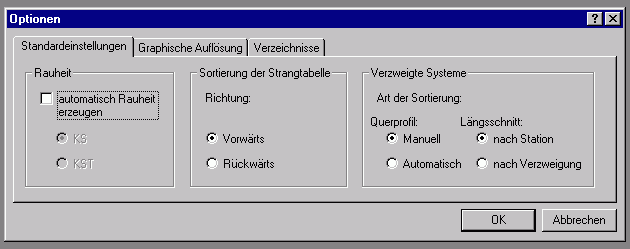
\includegraphics[width=0.9\linewidth]{extras_optionen}
   \caption{Benutzerdefinierte Einstellm�glichkeiten}
   \label{Installation Abb extras_optionen}
\end{figure}

\subsection{Standardeinstellungen}
\label{Installation Subsec Standardeinstellungen}

Beim Erstellen von Querprofilen besteht die M�glichkeit standardm��ig die Datens�tze Gel�ndeh�he, Trennfl�chen, Durchstr�mte Bereiche und Rauheiten automatisch anzulegen. Die Registerkarte Standardeinstellungen bietet Ihnen die M�glichkeit, festzulegen, welche Rauheiten, nach \autor{Darcy-Weisbach} oder \autor{Manning-Strickler}, hierf�r zugrundegelegt werden sollen (siehe auch Abschnitt~\ref{Einstieg Subsec Rauheit}). 

Ferner haben Sie hier die M�glichkeit die Art der Sortierreihenfolge f�r das Neuanlegen und Aufnehmen von Profilen festzulegen. Standardm��ig erfolgt die Sortierung der Strangtabelle von der niedrigsten zu h�chsten Station (Vorw�rts). Da einzelne Gew�sser aber auch von der M�ndung zu Quelle hin stationiert sind, haben Sie an dieser Stelle die M�glichkeit, die automatische Sortierreihenfolge umzukehren.

Weiterhin k�nnen Sie Festlegungen zur Sortierreihenfolge der Querprofile in verzweigten Systemen treffen (siehe hierzu auch Ab\-schnitt~\ref{Sonderprofile Sec VerzweigteSysteme}).


\subsection{Grafische Aufl\"{o}sung}
Hier k\"{o}nnen sie die Aufl\"{o}sung Ihres Bildschirms manuell einstellen. Die Voreinstellung steht auf automatischer Erkennung.
Die Darstellung der Masken ist optimal bei einer Grafikaufl\"{o}sung von $1024\times768~\mathrm{Pixel}$, wobei eine kleine
Schrift mit einer Skalierung von $100\%$ einzustellen ist.

\subsection{Verzeichnisse}
\label{Installation Subsec Verzeichnisse}
\begin{description}
   \item[Hauptverzeichnis:]
      Das Hauptverzeichnis wird immer dann ge\"{o}ffnet, wenn Sie ein neues Projekt anlegen. Geben Sie hier den Pfad zu dem
      Ordner ein, in dem sie normalerweise Ihre Projekte ablegen.
\end{description}
\begin{hinweis}
   Um Probleme beim Erstellen eines Projektes zu vermeiden, verwenden Sie keine langen Verzeichnisnamen mit Umlauten oder
   Sonderzeichen. M\"{o}chten Sie Ihre Projekte z.B. unter \datei{C:\textbackslash Eigene Dateien} ablegen, so verwenden Sie
   den DOS-Namen, beispielsweise \datei{C:\textbackslash Eigene$\sim$1}, des Verzeichnisses.
\end{hinweis}

\wspwin{} bietet die M\"{o}glichkeit, direkt aus der Oberfl\"{a}che heraus externe Programme zu starten. Damit \wspwin{} wei{\ss}, wo
sich Ihr Programm befindet, haben Sie hier die M\"{o}glichkeit, den entsprechenden Pfad anzugeben.
\begin{description}
   \item[Editor:]
      Geben sie hier den Pfad zu einem externen Texteditor ein. Dieser wird \"{u}ber das Men\"{u}
      \menu{\marrow \underline{E}rgebnisse \marrow \underline{E}ditor}
      aufgerufen.
   \item[CAD-Programm:]
      Geben sie hier den Pfad zu einem CAD-Programm an, das sie normalerweise verwenden. \"{U}ber das Men\"{u}
      \menu{\marrow P\underline{l}otten \marrow \underline{C}AD-Programm} k\"{o}nnen Sie das Programm starten und so von
      \wspwin{} erstellte dxf-Dateien bearbeiten.
   \item[Sonderprogramm:]
      Hier haben sie die M\"{o}glichkeit den Pfad f\"{u}r ein beliebiges externes Programm anzugeben, das aus \wspwin{} heraus
      gestartet werden soll. Der Programmaufruf erfolgt \"{u}ber den Men\"{u}punkt \menu{\marrow E\underline{x}tras \marrow
      \underline{S}onderprogramm}.
\end{description}


%%%%%%%%%%%%%%%%%%%%%%%%%%%%%%%%%%%%%%%%%%%%%%%%%%%%%%%%%%%%%%%%%%%%%%%%%%%%%%%%%%%%%%%%%%%%%%%%%%%%%%%%%%%%%%%%%%%%%%%%%%%%
\section{Deinstallation}
\label{Installation Sec Deinstallation}
%%%%%%%%%%%%%%%%%%%%%%%%%%%%%%%%%%%%%%%%%%%%%%%%%%%%%%%%%%%%%%%%%%%%%%%%%%%%%%%%%%%%%%%%%%%%%%%%%%%%%%%%%%%%%%%%%%%%%%%%%%%%

Windows~95/NT bietet die M\"{o}glichkeit der Deinstallation. Nach der Installation erscheinen im Startmen\"{u} unter dem
Programmgruppensymbol Spiegellinienberechnung (vgl. Abbildung~\ref{Einstieg Abb Programmstart}) zwei Eintr\"{a}ge:
\begin{quote}
   \menu{WSPWIN}, \"{u}ber das Sie das Programm starten k\"{o}nnen, und \\[6pt]
   \menu{UnInstallShield}, das es erm\"{o}glicht, die Software wieder zu l\"{o}schen.
\end{quote}
Die Eintr\"{a}ge in der Datei \datei{autoexec.bat} bleiben jedoch auch nach dem Ausf\"{u}hren des Deinstallationsprogramms
bestehen. Um sie zu entfernen, \"{o}ffnen sie die Dateien in einem Editor und entfernen die Eintr\"{a}ge von Hand. Danach m\"{u}ssen
sie den Computer neu starten.
